\documentclass[a4paper,man,natbib]{apa6}
\usepackage{microtype}
\usepackage{mathtools} % needed
\usepackage{hyperref}
\usepackage{tabularx}
\usepackage{lingex}
\usepackage[modulo,displaymath,pagewise]{lineno}

\newcolumntype{Y}{>{\raggedright\arraybackslash}X}
\usepackage[normalem]{ulem}
\hypersetup{hidelinks=True}
\newcommand*{\smex}[1]{\textit{#1}} % 'small example'
\newcommand*{\spex}[1]{``{#1}''} % 'spoken example'
\newcommand*{\term}[1]{\emph{#1}} % introducing a new term
\newcommand*{\citegen}[1]{\citeauthor{#1}'s~(\citeyear{#1})}
\newcommand*{\SE}{\mathit{SE}} % fix funny "SE" spacing
\newcommand{\resultsLog}[3]{$\beta = #1$, $\textnormal{SE} = #2$, $p #3$}
\newcommand{\resultsLM}[3]{$\beta = #1$, $\textnormal{SE} = #2$, $t #3$}

\usepackage[obeyFinal,textsize=tiny,backgroundcolor=yellow!60,linecolor=black!60]{todonotes} % to get rid of all notes, pass
% `final' to the document class
\setlength{\marginparwidth}{2cm}
\let\oldtodo\todo
\renewcommand*{\todo}[1]{\oldtodo[fancyline]{#1}}

\title{Such gesture, very lie, wow}
\author{reorder(MC,JK,JL)}
\affiliation{Psychology, PPLS, University of Edinburgh}
\ifapamodeman{\note{\begin{flushleft}%
Josiah King\\
Philosophy, Psychology and Language Sciences\\
University of Edinburgh\\
7~George Square\\
Edinburgh EH8~9JZ, UK\\[1ex]
\url{J.P.J.King@sms.ed.ac.uk}
\end{flushleft}}}

\abstract{
When questioning the veracity of an utterance, we perceive certain non-linguistic behaviours to indicate that a speaker is being deceptive.
Recent work has highlighted that listeners' associations between speech disfluency and dishonesty are detectable at the earliest stages of reference comprehension, suggesting that the manner of spoken delivery influences pragmatic judgements concurrently with the processing of lexical information.
Here, we investigate the integration of visual information about a speaker into judgements of deception.
By studying the time course of judgements of a speaker's (dis)honesty when presented with different visual cues to deception, we ask whether listeners are relying upon rule-of-thumb associations between visual cues and deception, or whether a link between gestures and perceived deception requires a more complex inferential process.
Participants saw and heard a video of a potentially dishonest speaker describe treasure hidden behind an object, while also viewing images of both the named object and a distractor object. 
Their task was to click on the object behind which they believed the treasure to actually be hidden.
Eye- and mouse-movements were recorded. 
Experiment~1 investigated listeners' associations between visual cues and deception, using a variety of static and dynamic cues.
Experiment~2 focused on adaptor gestures. 
We show that gestures can have a rapid and direct influence on pragmatic judgements, supporting the idea that communication is fundamentally multimodal.
\todo{JK: part of me has been trying to avoid using the term gesture as literature often doesn't count e.g. trunk movements as gestures}
%Although the nonverbal delivery of an utterance is found to influence the early stages of reference comprehension, establishing deception-judgements based on visual cues appears to be more gradual than previous studies have suggested it is for spoken cues.
}


\begin{document}

\shorttitle{What do liars look like?}
\maketitle
\linenumbers
\noindent
In natural communication, speakers can convey information via multiple channels.
Along with spoken delivery, a speaker's gestures, postures and facial expressions all offer information which can have a bearing on the non-literal (or pragmatic) interpretation of a message, for instance conveying emotion \citep{Busso2004, Gregersen2005}.
One such pragmatic interpretation is the judgement of a statement's veracity.
Research suggests that there are many aspects of nonverbal delivery which we, as listeners, believe to be \term{cues-to-deception}. 
In an analysis of 33~studies, \citet{Zuckerman1981} found that nine out of the ten visual cues-to-deception that were investigated were believed to be indicative of deceit. 
In a further subset of 13~studies reporting relationships between cues and subsequent deception judgements (rather than explicit beliefs about cues), three (smiling, gaze, and postural shifts) of the four available visual cues were associated with perceived dishonesty.

Interestingly, listeners appear to make these associations independent of the reliability of cues as actual signals of deception: \citet{Zuckerman1981} found only two visual cues (shrugs and fidgeting) to be associated with actual deceit, and a more recent meta-analysis found little evidence of a relationship between lying and almost any form of movement \citep{DePaulo2003}.
Some studies have in fact found deception to be inversely related to the cues we think of as deceitful:
Lying has been linked with a \emph{decrease} in hand, arm, and leg movements \citep[e.g.][]{DePaulo1992, Ekman1989, Vrij1995}, as well as a reduction in illustrative gesturing \citep[e.g.][]{DePaulo2003, Cohen2010}.
Even speakers' post-hoc perceptions of their own gestures when lying have been found to be at odds with how they actually behave:
\citet{Vrij1996} found that after partaking in interviews in which they were in turn truthful and dishonest, participants believed that their movements increased when lying, even though a decrease actually occurred.
An alternative view suggested by \citet{Hartwig2011} is that listeners are not relying on the wrong cues when forming judgements of deception, it is simply that associations between behavioural cues and lying are weak \citep{Hartwig2011}.

Whether listeners' intuitions about deceitful behaviour are misjudged or merely exaggerated, the associations they make between visual information and deception are unlikely to have been learnt.
This is reinforced by the fact that in everyday communication, there are few occurrences where listeners are given immediate feedback on the honesty of a given utterance.
Why do listeners associate certain behaviours with deceit, and how are they incorporated into the judgements listeners make about whether or not an utterance is true?
One suggestion is that listeners' judgements might follow simple and straightforward rules-of-thumb, relying on heuristically associating certain cues with deception \citep{DePaulo1982}.
The heuristics may be predicated on lay beliefs about deception, or on introspection as a speaker rather than experience as a listener.
For instance, if people believe that they themselves fidget more when they lie, they may be inclined to interpret fidgeting in others as cues to deception.
Following a rule-of-thumb like this would mean that listeners' judgements about whether or not someone is lying can occur quickly and with little effort.

\citet{Loy2017} investigated the association between lying and speech disfluency, and found support for the idea that listeners rely on rules-of-thumb when judging the veracity of an utterance based on the way in which it is spoken.
\citeauthor{Loy2017} used a visual world eye- and mousetracking paradigm in which participants were presented with images of two objects, and heard utterances describing the location of some treasure purportedly hidden behind one of the objects.
These utterances were presented as having been elicited in a previous experiment, in which the speaker was said to have been lying some of the time.
Crucially, \citet{Loy2017} manipulated the manner of spoken delivery, with half of the experimental items containing a speech disfluency.
Participants were tasked with clicking on the object they \textit{believed} to be concealing the treasure, choosing either the object named in the utterance (indicating a judgement of honesty), or a distractor (dishonesty).
They were more likely to judge disfluent utterances as dishonest than fluent ones (as indicated by a greater probability of clicking on the distractor in a disfluent trial). 
Importantly, disfluency resulted in an early bias in both eye and mouse movements towards the not-referred-to object.
This suggests that speech disfluency is already incorporated into listeners' ideas concerning deceptive speech, and has an immediate effect on their interpretation of an utterance. 

It seems reasonable to assume that the early effects of speech disfluency reflect a rule-of-thumb association of disfluency with dishonesty.
In fact, any rule-of-thumb may be quite general:  Evidence suggests, for example, that some effects of speech interruptions on comprehension are not sensitive to differences between a spoken \spex{um} and an artificial tone \citep{Corley2011}.
Co-speech movements, however, are substantially more varied than speech interruptions, serving as both potential markers of metacognitive states and planning processes, and as an alternative modality in which a speaker can convey semantic information \citep[See, e.g.][]{Ekman1969,Mcneill1992}.
Any rule-of-thumb linking visual information to deception would have to be refined enough to discriminate types and contents of co-speech movements, or risk potentially over-attributing any cue as a sign of deceit.
Furthermore, listeners associate static visual cues with deception \citep[e.g. eye-gaze,][]{Zuckerman1981a}, suggesting that judgements of dishonesty are not linked just to variations in movement, but to a wide array of visual cues. 

An alternative to the heuristic explanation suggests that non-linguistic information might influence listeners' judgements of deception via a form of on-the-fly speaker modelling: 
When presented with a possibly deceitful utterance, listeners might be inferring information about a speaker's metacognitive states, linking visual and spoken cues to deception via the perception of, e.g., nervousness, or cognitive effort. 
Such an account requires more complex inferential processing.
Participants would have to make links between specific visual cues and metacognition, which would in turn be linked to a judgement of veracity.

To date, the link between visual cues and perceived deceit has been studied only in terms of after-the-fact judgements, or assessing listeners' explicit beliefs about cue validity (see \citealt{Vrij1996a, Zuckerman1981a}).
In the two experiments presented here, we extend the `treasure game' paradigm from \citet{Loy2017} to include a video of a potentially deceptive speaker describing the location (behind one of two objects) of some hidden treasure on the screen (see Figure \ref{fig:v1_layout}).
Crucially, we manipulate the presence or absence of potential visual cues to deception in the video.
Listeners attempt to guess, and click on, the true location of the treasure, which allows us to infer whether they believe the speaker to be lying or telling the truth.
If listeners associate a given visual cue with deception, they should be more likely to click on the object which has not been mentioned.
By measuring listeners' eye- and mouse-movements as the speaker's descriptions unfold, we can investigate their interpretations of what is being said over time.
%To the extent that this bias occurs early during relevant trials, it is possible to infer that listeners are acting on a heuristic association between cue and falsehood.

\begin{figure}[Ht]
  \centering
	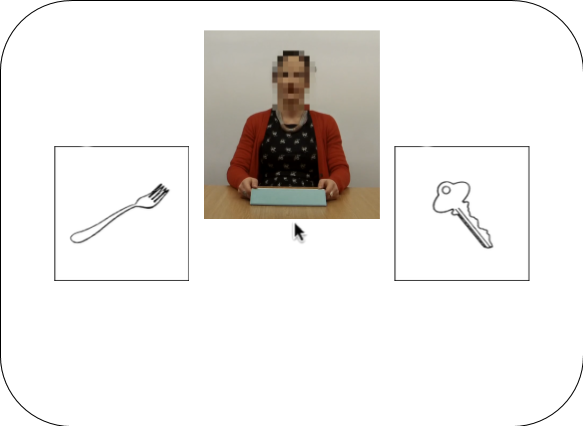
\includegraphics[width=\linewidth]{./img/e7_layout.png}
  \caption{Visual world with video stimulus}
  \label{fig:v1_layout}
\end{figure}

In Experiment~1, we focus on how trunk movements (postural shifts) influence judgements of utterance veracity, with filler trials presenting two further types of visual cue (adaptor gesturing, and different static postures).
The decision to focus on trunk movements had two bases: Firstly, previous research indicates that these movements are associated with perceived lying \citep{Vrij1996a}, and secondly, they offer practical advantages in integrating a video stimulus into the visual-world paradigm, as we require visual cues to be salient enough for participants to notice them, but not to detract from fixations to objects at the auditory onset of the critical noun.
Trunk movements involve larger movements than hand or head movements, and appear believable when presented with little or no overlap with the spoken words of an utterance, providing a visual cue comparable to the utterance-initial disfluency in \citet{Loy2017}.
Because effects emerged for the fillers in Experiment~1, we conducted Experiment~2 as a replication, focused exclusively on adaptor gestures.


\section{Experiment~1}
Experiment~1 makes use of eye- and mouse-tracking to investigate whether visual cues affect listeners' judgements about the veracity of an utterance over time. 
The experiment was presented as a `lie detection game'.
Each trial included a video and audio recording of a potentially deceptive speaker describing the location of some hidden treasure.
Throughout a trial, two images, depicting potential treasure locations, remained visible on the screen. 
Participants were tasked with using the mouse to click on the object they believed to be concealing the treasure.
Critical trials presented videos of the speaker either producing a trunk movement immediately prior to utterance playback, or sitting motionless (no cue) for the equivalent amount of time.
Filler trials presented videos of the speaker producing no cue, sitting in a different posture, or producing an adaptor gesture. 
Our aim was to investigate whether and when gestural cues would be associated with falsehood.
%% (add) Our results show that...

\subsection{Participants}
Twenty-four self-reported native speakers of English were recruited from the University of Edinburgh community, and took part in the experiment in return for a payment of \pounds{}4.
Participants all had normal or corrected-to-normal vision, and were all right-handed mouse users.

\subsection{Materials}
Visual stimuli consisted of the same 120 line drawings from \citet{Snodgrass1980} which were used in \citet{Loy2017}, sixty of which served as the object named as hiding the treasure and the other sixty as distractors.
Referents were randomly paired with distractors and presented across sixty trials (20 critical and 40 fillers). 
Following \citet{Loy2017}, critical referents and distractors had been matched for both ease of naming and familiarity.
In each trial, the speaker named one object (referent) as that which concealed the treasure; the other object is hereafter named the distractor.
Each referent was associated with a recording of fluent speech specifying the image as the object that the treasure was hidden behind (``The treasure is behind the <referent>'').
Trials also presented a video of a person who was purported to be the speaker of the utterances. 
Videos showed the person speaking and either producing a gestural cue or sitting motionless in a neutral posture.
The face shown in the video was pixelated, to allow videos to be presented alongside different utterances and maintain the illusion that for each trial the spoken utterance heard was the corresponding audio track captured with the video (and produced by the person in the video).


Thirty-five videos were created by asking a volunteer to repeat the phrase \spex{The treasure is behind the <object>} (ensuring that when videos were subsequently edited to pixelate the face, pixel movement maintain loosely patterned with the length of utterances presented to participants).
%JK swap the below for the above?
%Thirty-five videos were created
Ten of these showed a speaker sitting motionless with her hands on either side of a tablet computer (upon which the referent, distractor, and treasure was purported to be displayed) which was resting on a table.
These ten videos were each seen in one critical trial, and repeated in two filler trials.
Five videos of trunk movements were each presented in two critical trials each.
The remaining 20 videos (each presented in one filler trial) showed the speaker either producing an adaptor gesture, such as finger-tapping or head-tilting, (10 videos) or sitting motionless but in a different, non-neutral posture, such as hand-on-chin or arms crossed (10 videos).
This meant that over the course of the experiment each participant saw 30 videos of the speaker producing no cue, and 30 videos of the speaker producing some type of cue (10 showing trunk movements; 10 showing adaptor gestures; 10 showing different postures).

We identified a timepoint in each video at which, according to our judgement, it would be natural for audio to begin. 
For videos showing a trunk movement, this was the frame of the video at which the movement ended, meaning that participants were presented with no overlap between the movement and speech.
These were matched in videos showing no cue, thus controlling for any sensitivity to the duration of video prior to speech (which could be interpreted as speech-initiation time, in turn a potential cue to deception). 
For videos showing an adaptor gesture the amount of overlap between visual cue and varied, and was matched in videos showing the speaker in different static postures.

As with \citet{Loy2017}, 20 critical referents were counterbalanced across two lists. 
Each list contained 10 trials showing a trunk movement video and 10 trials showing a video showing no cue.
The remaining 40 referents were randomly paired with one of the remaining videos (10 showing adaptor gestures, 10 showing different postures, 20 showing no cue) for each participant, with no repetition of referents across videos.

\subsection{Procedure}
The experiment was presented using OpenSesame version~3.1 \citep{Mathot2012}.
Stimuli were displayed on a 21~in.\@ CRT monitor with a resolution of 1024~$\times$~768, placed 850~mm from an Eyelink~1000 Tower-mounted eye-tracker which tracked eye movements at 500~Hz (right eye only). 
Audio was sampled at 44100~Hz and presented in stereo from speakers on either side of the monitor. 
Videos were presented at 25~fps, and mouse-coordinates were sampled equivalently (every 40~ms).
Eye movements, mouse coordinates and object clicked (referent or distractor) were recorded for each trial.

Figure \ref{fig:v1_trial} represents a sample trial from the experiment. 
Between trials, participants underwent a manual drift correction to ensure accurate recordings from the eye-tracker.
After this the central fixation dot turned red for 500ms to signify progression to the trial. 
This was replaced by two images corresponding to the referent and distractor, each measuring 150~$\times$~150 pixels, centered vertically and positioned such that the center of each object was 15\% from either edge of the display. 
The relative positions (left vs.\@ right) of referents and distractors was randomly chosen, with the constraint that each participant saw the referent in an equal number of critical and filler trials on the left as on the right.
This display of two images lasted for 2000~ms before the video was added and the cursor was centred and made visible.
The video, measuring 266~$\times$~284 pixels, was displayed with the bottom edge at the vertical midpoint of the screen, and centered horizontally.
Playback of the utterance began at the assigned frame of the video.
The trial ended once the participant clicked on either object, or 5000~ms after the onset of the referent noun.

\begin{figure}[Ht]
  \centering
	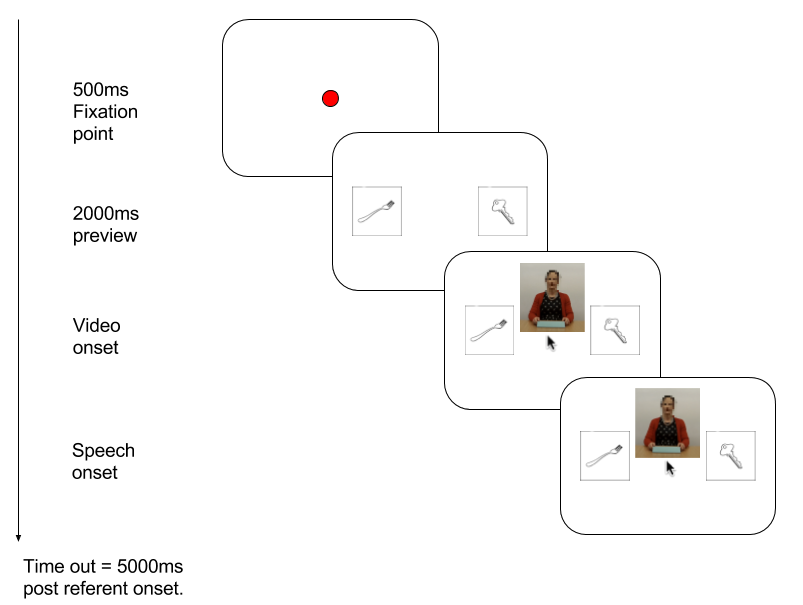
\includegraphics[width=\linewidth]{./img/e7_trial.png}
  \caption{Procedure of a given trial, Experiment~1}
  \label{fig:v1_trial}
\end{figure}

Participants were told that the videos they saw were recordings taken from a previous experiment, in which one participant was tasked with describing the location of some hidden treasure with the aim of misleading the other participant into choosing the wrong location.
To emphasise this, participants were shown a staged photograph of two people purportedly participating in this previous experiment. 
Participants were told that the speakers in the previous experiment would lie approximately half of the time. 
Participants were instructed to click on the object behind which \textit{they believed} the treasure to be hidden, with the overall aim of accumulating as much treasure as they could across the experiment.
Participants received no feedback after their object clicks, except on bonus trials, which are described in the next section.

The order of trials was randomly assigned on each run of the experiment.
Participants completed five practice trials (one of which was presented as a bonus round) prior to the main experiment. 
Two of these presented a video showing no cue, two displayed a video of the speaker in different postures, and one displayed a video of the speaker making a trunk movement.


\subsection{Bonus Trials}
To maintain motivation throughout the study, participants were told that there were a number of ``hidden bonus rounds'' which offered more treasure than regular rounds.
25\% of filler trials (half presenting a video showing either adaptor gesturing or a different posture; half presenting a video showing no cue) were randomly designated as bonus rounds for each participant.
These trials were visually identical to regular trials.
However, following the mouse click (regardless of the object chosen), a message was displayed informing participants that they had successfully located bonus treasure.
Participants were told that the top scorers would be able to enter their names on a high-score table, which was shown at the beginning of the experiment. 

\subsection{Post-test Questionnaire}
Participants were asked to complete a short post-test questionnaire which asked whether participants had noticed anything odd about the visual or audio stimuli.
Any participant who indicated that they had noticed anything unusual was then questioned further, to decide whether they believed that the speech and gesture had been produced naturally and simultaneously.
All participants were subsequently debriefed, during which they were told that the audio and video were created separately and stitched together, and asked again verbally if they noticed anything unusual in that respect. 
Responses to the questionnaire and debrief were used to determine whether participants should be excluded from the analysis.

\section{Results}

\subsection{Analysis}
Analysis of critical trials was carried out in R version~3.4.4 \citep{Rbase2017}, using the lme4 package version~1.1-17 \citep{Bates2015}. 
Data from four participants who indicated suspicion of the supposed origins of the audiovisual stimuli based on the post-test questionnaire and/or debrief were removed from all analyses, leaving data from Twenty participants. 
Of 400 critical trials, one trial in which participants did not click on either the referent or distractor was excluded from all analyses.
%JK mouse samples removed?

Object clicked (referent or distractor) was modelled using mixed effects logistic regression, with a fixed effect of visual cue (no cue vs.\@ trunk movement), deviation coded, with random intercepts and slopes for visual cue both by-participant and by-item.
Reaction times (measured from referent onset) were log transformed and modelled with the same fixed and random effect structure using mixed effects linear regression.

Eye fixation data was averaged into 20~ms bins (of 10 samples) prior to analysis.
For each bin, we calculated the proportions of time spent fixating the referent or the distractor, resulting in a measure of the proportions of fixations on either object over time.
The position of the mouse was sampled every 40~ms.
Using the $X$ coordinates only, we calculated the number of screen pixels moved and the direction of movement (towards either referent or distractor).
We then calculated the cumulative distance travelled towards each object over time as a proportion of the cumulative distance travelled in both directions from referent onset up until that time bin.
Movements beyond the outer edge of either object were considered to be `overshooting' and were not included in calculations (0.8\% of samples).
Eye- and mouse- biases were calculated from the proportions of referent to distractor fixations, and were subsequently empirical logit transformed \citep{Barr2008}. 
In these measures, a value of zero indicates no bias towards either object, and positive and negative values indicate a bias towards the referent and distractor respectively.

As in previous studies using the treasure game paradigm \citep{King2018,Loy2017}, eye- and mouse- tracking analyses were conducted on a time-window beginning at referent onset and extending for 800~ms, just beyond the duration of the longest referent (776~ms).
Eye and mouse data was modelled over this time window using linear mixed effects models, with fixed effects of time from referent onset (seconds), visual cue (deviation coded), and their interaction.
Random intercepts and slopes for time and visual cue were included both by-item and by-participant, with the addition of a by-participant interaction between time and visual cue.
Following \citet{Baayen2008}, we considered effects in these models to be significant where $|t|>2$.

\subsection{Object clicks}
Across the experiment, participants clicked on the referent in 56\% of critical trials and the distractor in 44\%.
Table \ref{table:v1_clicks} shows the percentage of clicks across all participants to either object following videos showing different types of cue.

Analysis of critical trials indicated that visual information about the speaker had marginal effects on participants' decisions to click on either object, with videos showing no cue resulting in marginally more clicks on the referent (\resultsLog{0.56}{0.32}{=0.08}).
There was no effect of visual cue on the time taken by participants to click on an object.

\begin{table}
\caption{Breakdown of mouse clicks in critical trials recorded on each object (referent or distractor) by type of visual cue for Experiment~1}
\label{table:v1_clicks}
\begin{tabularx}{\linewidth}{YYYYY}
\hline
& No Cue & Trunk Movement \\
Clicks to Referent & 125 (62.5\%) & 99 (49.7\%) \\ 
Clicks to Distractor & 75 (37.5\%) & 100 (50.3\%) \\
\hline
\end{tabularx}
\end{table}

\subsection{Eye movements}
Figure \ref{fig:v1_eye1} shows the time course of fixations to referents and distractors in critical trials for the 2000~ms from referent onset, split by whether the video showed either no cue or a trunk movement.
Analysis of critical trials conducted over the 800~ms period from referent onset showed a main effect of time (\resultsLM{2.40}{0.69}{=3.65}) indicating that participants tended to fixate on the referent over the distractor more as time from referent onset increased.
There were no main effects of visual cue, nor any interaction of visual cue with time, indicating that participants tendency to fixate upon the referent was not influenced by whether the video showed the speaker producing a trunk movement or sitting motionless.

\begin{figure}[Ht]
  \centering
	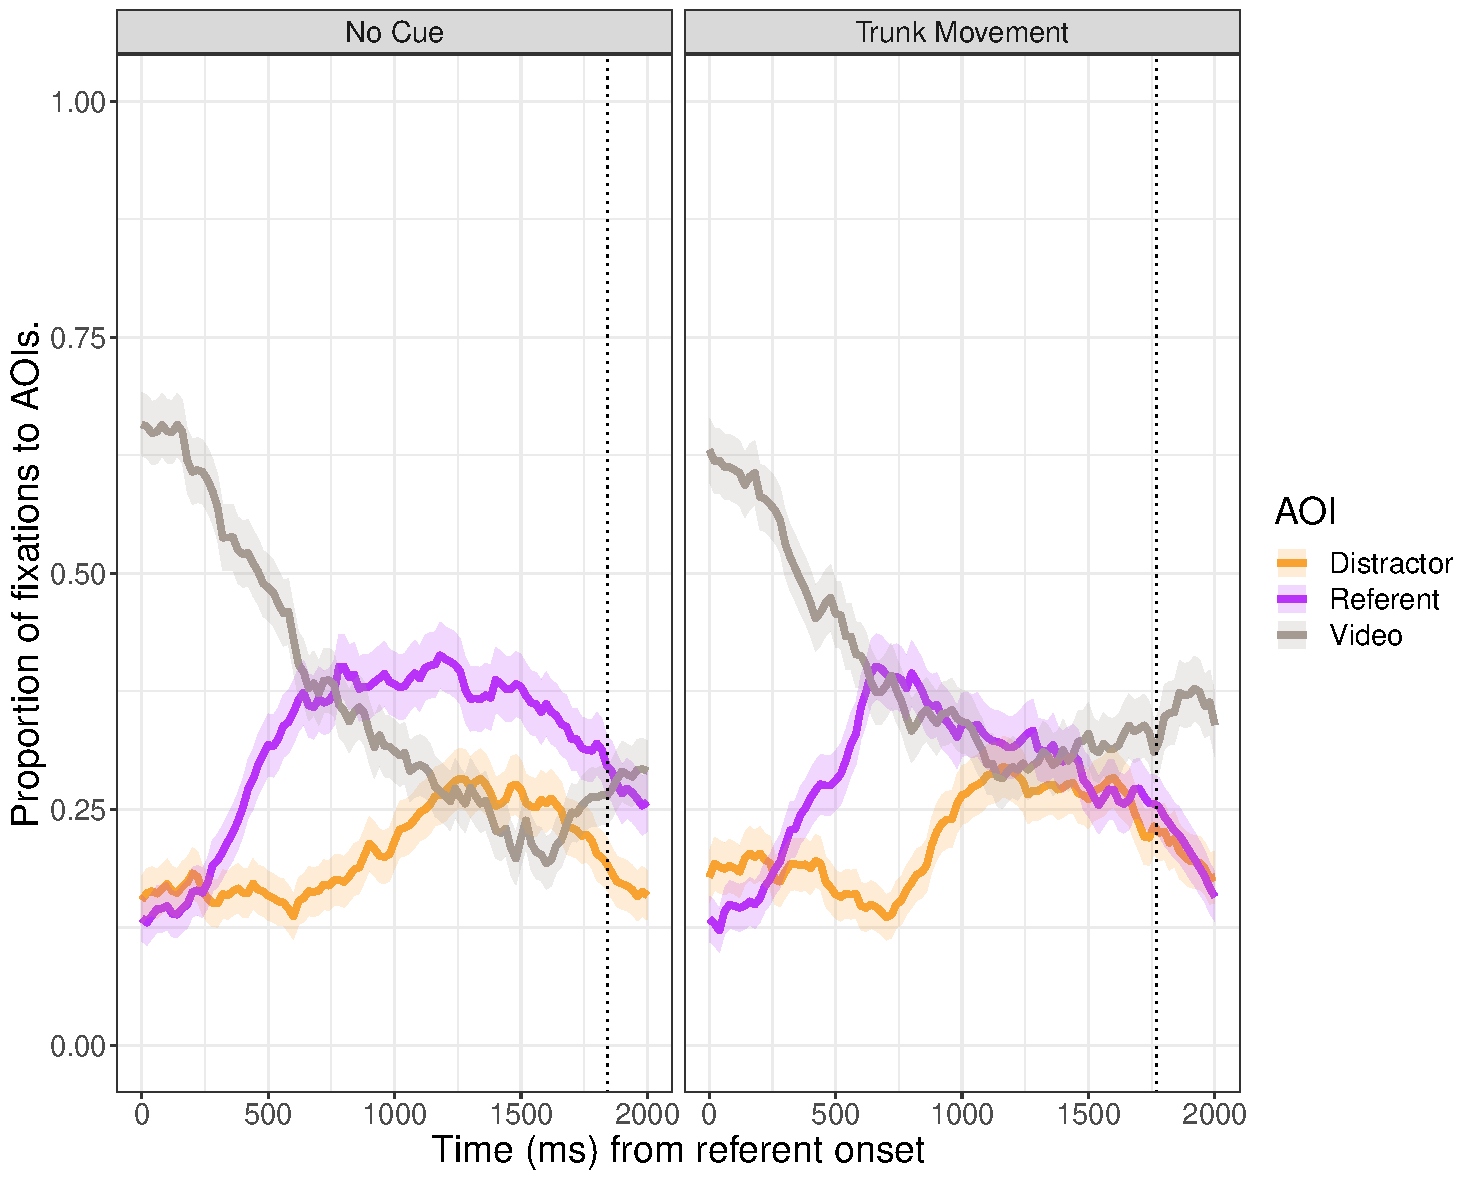
\includegraphics[width=\linewidth]{./img/e7_fixations_crit.pdf}
  \caption{Eye-tracking results for critical trials in Experiment~1: Proportion of fixations to each object (referent or distractor) and the video, from 0 to 2000 ms post-referent onset, calculated out of the total sum of fixations for each 20~ms time bin. Shaded areas represent $\pm$ 1 standard error of the mean.}
  \label{fig:v1_eye1}
\end{figure}

\subsection{Mouse movements}
Figure \ref{fig:v1_mouse1} shows the time course of the proportions of cumulative distance the mouse moved towards the referent and distractor in critical trials for 2000~ms from referent onset, split by whether the video showed either no cue or a trunk movement.
Analysis on the 800~ms following referent onset showed that participants' mouse-movements patterned with their eye-movements:
Participants tended to move the cursor towards the referent over the distractor more as time increased (\resultsLM{0.73}{0.32}{=2.31}), and there was no main effect of visual cue nor an interaction of visual cue with time.

\begin{figure}[Ht]
  \centering
	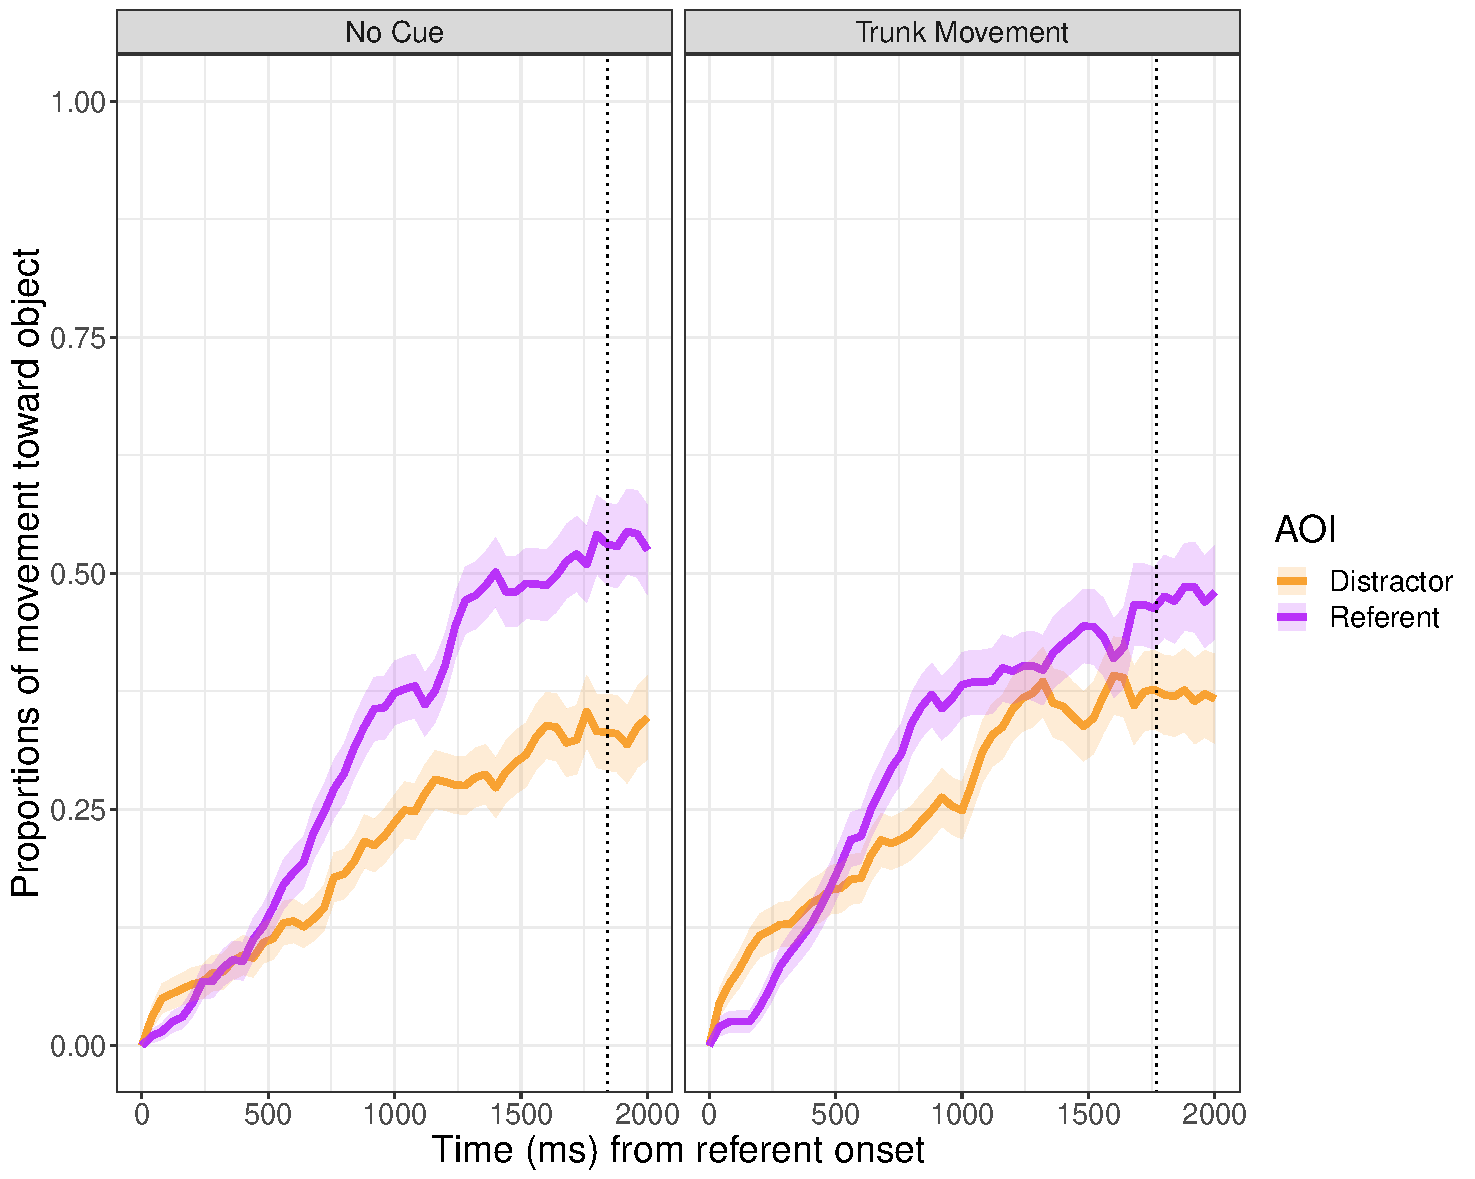
\includegraphics[width=\linewidth]{./img/e7_mouse_crit.pdf}
  \caption{Mouse-tracking results for critical trials in Experiment~1: Proportion of cumulative distance traveled toward each object from 0 to 2000 ms post-referent onset. Proportions were calculated from the total cumulative distance participants moved the mouse until that time bin (from video onset, when cursor was made visible). Shaded areas represent $\pm$ 1 standard error of the mean.}
  \label{fig:v1_mouse1}
\end{figure}

\section{Discussion}
Experiment~1 investigated how the pragmatic inferences listeners make about a speaker's honesty are influenced by the presence of visual cues to deception in the form of trunk movements.
We measured eye- and mouse- movements of participants who were presented with a task in which they made decisions about the true location of some treasure based on audio and video of a potentially deceptive speaker making a statement about the treasure's location.
Participants were thus making implicit decisions about the honesty of each utterance.
As in previous studies using versions of this paradigm \citep{Loy2017, King2018}, participants showed an overall tendency to interpret an utterance as truthful.
Whether the videos which were presented alongside utterances showed the purported speaker producing a trunk movement or sitting motionless had no effect on participants' judgements of deception.
Participants' eye- and mouse- movements during the 800~ms following referent-onset were likewise not influenced by whether the video showed a trunk movement or no cue.


Post-hoc analysis of filler trials, however, indicated that for trials which showed a video of the speaker producing adaptor gesture, participants tended to click more on the distractor.
Furthermore, 
%JK bit about online effects


Overall, these findings contrast with our prediction that trunk movements would provide the best opportunity to investigate the association between visual cues and deception-judgements.
One possible explanation for the failure of videos showing trunk movements to elicit judgements of deception could be due to the fact that at the point of referent onset, the audiovisual information immediately available to the listener was comparable to the videos showing no cue (trunk movements having ended at speech onset).
Comparatively, despite the cues used in filler trials showing movement in a smaller area of the video (or no movement at all), their proximity in time to critical noun may explain why they, but not trunk movements, appeared to elicit judgements of deception. %JK both, or just adaptors?
This explanation, however, is at odds with the bias towards judgements of deception following utterance-initial disfluencies observed in previous work \citep[][Experiment~1]{Loy2017}.
We cannot at present reconcile this discrepancy, although it may point towards different visual cues having different effects on judgements of deception---something which is supported by comments from several participants in the post-test questioning that they based their judgements on \spex{how relaxed the speaker looked}.

Results from Experiment~1 do not support previous findings that addressees associate trunk movements with lying: When viewing a potentially deceitful speaker, the presence of a trunk movement immediately prior to speech was not found to influence addressees' judgements of (dis)honesty. 
However, additional analyses of filler trials in which videos showed the speaker producing either an adaptor gestur or sitting in a different posture indicate that these behaviours (specifically adaptor gesturing) may be associated with perceived lying.
Furthermore, the results of post-hoc analyses on eye- and mouse- movements in filler trials suggest that this association may be detectable at the early stages of reference comprehension. 
From a practical viewpoint, this suggests that the visual world paradigm may be compatible with a range of video stimuli, including those in which movement co-occurs with speech: For instance, videos showing adaptor gesturing simultaneously with utterance playback did not stop a fixation bias appearing in the early stages of reference comprehension, and small movements such as finger tappings were salient enough to influence judgements of deception.

To directly investigate the association between adaptor gesturing and perceived dishonesty, we conducted Experiment~2, in which participants saw videos of a speaker either producing an adaptor gesture, or sitting motionless, and there were no filler trials.

\section{Experiment~2}
Using the same paradigm as Experiment~1, participants in Experiment~2 heard utterances accompanied by a video of a speaker either producing an adaptor gesture or sitting motionless, and were tasked with making an implicit judgement on whether the speaker was lying or telling the truth.
Videos in Experiment~2 showed adaptor gestures which have previously suggested to be associated with nervousness \citep[See][]{Gregersen2005}, and videos were pre-tested for perceived anxiety in the speaker.
As a manipulation check, after the treasure-game task, participants were asked to rate how nervous the speaker looked in each video (without audio).

\subsection{Participants}
Twenty-three self-reporting native English speaking participants took part in exchange for \pounds{}3 compensation.


\subsection{Materials}
The 40 images used in critical trials in Experiment~1 (20 referents; 20 distractors) were used across twenty trials.
As in Experiment~1, these images were displayed in referent-distractor pairs, with each pair shown alongside a recorded utterance naming the referent as the location of the treasure.
The pairing of referents and distractors on each trial was randomised.

As in Experiment~1, each pair of images and recorded utterance was presented alongside a video clip of a person purported to be the speaker of the utterance.
Twenty-eight new video clips were recorded (18 different adaptor gestures; 10 no-cue). 
Care was taken to ensure that the videos including no cue showed the speaker in a relaxed posture. 
Adaptor gestures were based on descriptions of anxious nonverbal behaviour from \citet{Gregersen2005}.
All 28 videos were pre-tested for perceived nervousness of the speaker.
Ten native english speakers were told that they were going to watch videos (without audio) of someone being questioned in a stressful situation, and were asked to rate how nervous the speaker looked in each video (1: very relaxed, 7: very nervous). 
The 10 videos showing adaptor gestures with the highest ratings (Mean = 4.1, SD = 1.5) were included in the experiment, along with the 10 videos showing no cue (Mean = 1.9, SD = 1.1).

The 20 referents were counterbalanced across two lists such that each referent that occurred with a video showing adaptor gesturing in the first list occurred with a video showing no cue in the second.
The pairings of referents with specific videos within each condition was randomised on each run of the experiment.

\subsection{Procedure}
The experiment procedure was identical to that of Experiment~1 with the following changes.
First, the size of the video stimuli changed slightly, and measured 236~$\times$~336 pixels.
Second, the duration of video presented prior to audio playback was set at a fixed constant (1400~ms).
Third, we did not include any `bonus' trials, so participants did not receive any feedback during the experiment.

After the main task, participants were asked to watch all 20 videos again, without audio, and asked to rate how nervous they thought the speaker looked (using the same 1-7 scale as described above).
Participants then completed the same post-test questionnaire as in Experiment~1, with data being excluded from analysis on the same basis.

\section{Results}
Data from three participants were excluded due to suspicion of the audiovisual stimuli being scripted (based on the post-test questionnaire and questioning during debrief), and analysis was conducted on data from the remaining 20 participants.

\subsection{Analysis}
We followed the same analysis strategy as was used for Experiment~1.
Trials which did not result in a click to either object (3) were excluded from analyses, leaving 397 trials.
Mouse-movements beyond the outer edge of either object were excluded from analyses (1\% of samples).
Analyses was identical to that of the critical trials in Experiment~1.

\subsection{Object clicks}
Across the experiment, participants clicked on the referent in 53\% of trials and the distractor in the remaining 47\%.
Table \ref{table:v2_clicks} shows the proportions of clicks to either object following videos showing either no cue or adaptor gesturing.
The presence of adaptor gesturing was found to influence participants' decisions to click on an object, with videos presenting adaptor gesturing resulting in more clicks to the distractor \resultsLog{-2.78}{0.38}{<0.001}.
The time participants took to click on an object was not influenced by whether the video showed an adaptor gesture or no cue.

\begin{table}
\caption{Breakdown of mouse clicks recorded on each object (referent or distractor) by cue type for Experiment~2}
\label{table:v2_clicks}
\begin{tabularx}{\linewidth}{YYY}
\hline
& No Cue & Adaptor gesture \\
Clicks to Referent & 161 (80.9\%) & 48 (24.2\%)  \\
Clicks to Distractor & 38 (19.1\%) & 150 (75.8\%)  \\
\hline
\end{tabularx}
\end{table}


\subsection{Eye movements}
Figure \ref{fig:v2_eye} shows the time course of fixations to referents and distractors over 2000~ms from referent onset, split by whether the video showed no cue or adaptor gesturing.
Analyses conducted over the time window of 800~ms post-referent onset revealed an interaction between time and cue (\resultsLM{-2.99}{0.71}{=-4.20})

a main effect of time (\resultsLM{1.52}{0.66}{=2.30})
There was a main effect of cue (\resultsLM{0.76}{0.31}{=2.47}) and an interaction between the cue and time, with adaptor gesturing attenuating the  (\resultsLM{-2.99}{0.71}{=-4.20})

\begin{figure}[Ht]
  \centering
	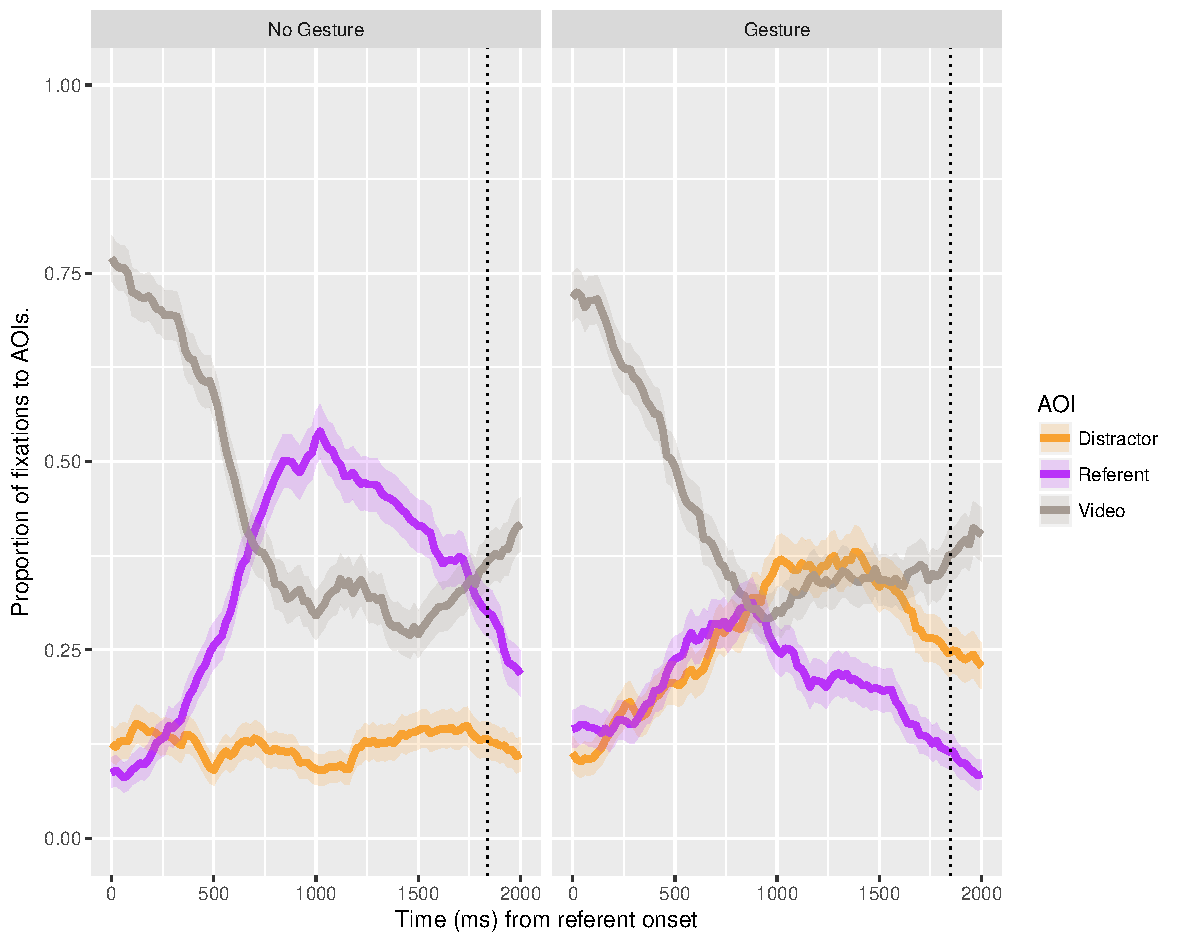
\includegraphics[width=\linewidth]{./img/e8_fixations.pdf}
  \caption{Eye-tracking results for Experiment~2: Proportion of fixations to each object (referent or distractor) and the video, from 0 to 2000 ms post-referent onset, calculated out of the total sum of fixations for each 20~ms time bin. Shaded areas represent $\pm$ 1 standard error of the mean.}
  \label{fig:v2_eye}
\end{figure}

\subsection{Mouse movements}
Figure \ref{fig:v2_mouse} shows the time course of the proportions of cumulative distance the mouse moved towards the referent and distractor for 2000~ms from referent onset, split by cue type.
Mouse-movements over the course of the 800~ms window from referent onset again patterned with the eye-tracking data:
Following videos showing no cue, participants showed a tendency to move the mouse increasingly towards referent over this period (\resultsLM{1.77}{0.31}{=5.72}), but this increasing referent-bias was greatly reduced following videos showing an adaptor gesture (\resultsLM{-2.16}{0.19}{=-11.40})

\begin{figure}[Ht]gesture
  \centering
	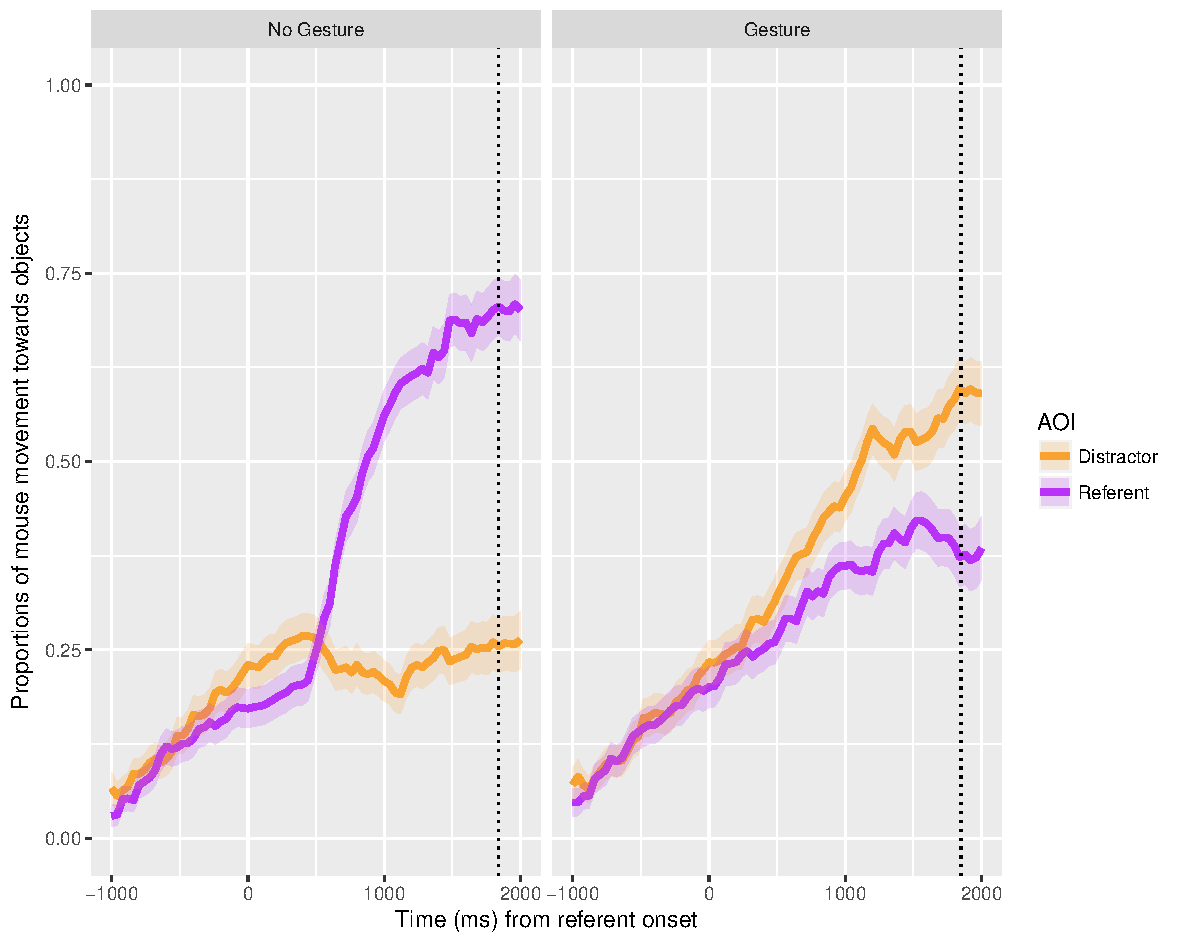
\includegraphics[width=\linewidth]{./img/e8_mouset.pdf}
  \caption{Mouse-tracking results for Experiment~2: Proportion of cumulative distance traveled toward each object from 0 to 2000 ms post-referent onset. Proportions were calculated from the total cumulative distance participants moved the mouse until that time bin (from speech-onset, when cursor was made visible). Shaded areas represent $\pm$ 1 standard error of the mean.}
  \label{fig:v2_mouse}
\end{figure}


\section{General discussion}
The studies presented here investigate the integration of visual information about a speaker into judgements of deception.
We manipulated the presentation of the different non-verbal behaviours while measuring eye- and mouse- movements of the listener towards one of two possible final judgements about the veracity of an utterance.
In doing so, we explored the possibilities of whether listeners are relying upon a rule-of-thumb heuristic in associating visual cues to deception, or whether the link between nonverbal behaviour and perceived deception requires a more complex inferential process.

In Experiment~1, listeners' final interpretations of utterance veracity were influenced by visual information about the speaker which was presented concurrently with presentation of speech.
However, these findings were only apparent in relation to visual cues used in filler trials (in which videos showed a speaker in different postures and producing adaptor gestures), with a marginal effect of the trunk movements which were the focus of the study.
Analysis of the filler trials in Experiment~1 indicated that visual information about a speaker can be integrated into the early stages of reference comprehension, and that this information can be both static and dynamic.
Experiment~1 also showed that the visual world paradigm can be adapted to include video stimuli of the speaker without detracting from fixation-biases, even when this video stimuli is changing during the presentation of speech.
This aligns with research suggesting that listeners may extract information about gestures through peripheral vision \citep[See e.g.][]{Gullberg2006}.
To directly investigate the time-course of judgements based on adaptor gestures in a fully counterbalanced design, we conducted Experiment~2, which confirmed that participants engaged in rapid integration of visual information into pragmatic judgements of deception.

The findings presented here are consistent with previous research on beliefs about and judgements on visual cues to deception showing that listeners perceive a range of nonverbal behaviours to indicate deceit \citep[e.g.][]{Zuckerman1981, Akehurst1996, Vrij2000}, and provides a visual-modality parallel with the findings from \citet{Loy2017} showing that fluency of speech influences judgements of whether a speaker is lying
Our findings, together with those from \citet{Loy2017}, suggest that listeners may have an implicit bias to judge a speaker as honest in the absence of any obvious potential cue to deception. 
Additionally, they align with the `truth bias' commonly observed in deception literature, in which listeners have a tendency to judge a speaker as truthful, even when explicitly told the speaker may be dishonest \citep{Vrij2000}.

The time course of listeners' eye- and mouse-movements showed that the influence of the visual channel is apparent during the early stages of comprehension:
In both experiments, utterances presented with the speaker in a neutral posture and not gesturing biased listeners towards believing the speaker to be truthful, as shown by increased tendency to fixate on, move the mouse towards, and eventually click on the object which was named by the speaker. 
In contrast, utterances presented alongside a visual cue such as an adaptor gesture significantly reduced this bias, as evidenced in Experiment~2.
Importantly, this difference emerged during the initial stages of linguistic processing, with effects found in Experiment~2 during the same time-window as that in which \citet{Loy2017} found effects of speech disfluency.
Just like manner of spoken delivery, the manner of visual delivery can very quickly modulate a listeners' judgements about the speaker's intentions alongside processing of the lexical information. 

Although it is tempting to interpret these results as indicative of participants relying on heuristically associating visual cues with lying, visual inspection of the time course suggests that this might not be the case.
When presented with a video showing a speaker producing an adaptor gesture, the bias towards the distractor --- signifying perceived dishonesty --- over the referent appeared approximately 1000~ms after the referent began, at a later point than previous versions of this paradigm in which speech disfluencies were found to modulate judgements of deception. 
This time course of events is difficult to reconcile with a view that listeners are relying on rule-of-thumb associations between visual cues and deception, and could suggest that listeners may be engaging in a more complex reasoning process in integrating manner of visual delivery than manner of spoken delivery. 

Our results show that the integration of the visual channel in utterance processing can have a rapid and direct effect on a listener's pragmatic judgements, supporting the idea that communication is fundamentally multimodal: 
Speech and gesture interactively codetermine meaning.
However, the integration of visual cues to inform deception judgements appears to be more gradual than the integration of spoken cues.
To better understand how information in different modalities affect comprehension, further research would require investigating the effect of spoken delivery when the visual channel is also available --- for example, studying the time course of deception judgements when faced with one or both of a disfluency and an adaptor gesture.


\bibliography{./GCD}

\end{document}



















%%%%%%%%%%%%%%%%%%%%%%%%%%%%%%%%%%%%%%%%%%%%%%%%%%%%%%%%%%%%%%%%%%%%%%

\section{Filler trials}

Filler trials (numbering 800) were analysed in the same way, with two differences. 
Firstly, in all models, by-item random effects for visual cue (Now comprising three levels: no cue, different postures, and adaptor gesturing) were removed as they were not counterbalanced across referents.
Secondly, eye- and mouse- tracking analyses was extended to 1100~ms following onset of the referent. 
This decision was based on the fact that the longest referent in filler trials was 1062~ms. 
Filler trials resulting in no mouse click on either object (n=3) were excluded from these analyses.
%JK mouse samples removed?

\subsection{Object clicks} 
Across the experiment, participants clicked on the referent in 55\% of filler trials and the distractor in 45\%, matching the clicks recorded in critical trials
Table \ref{table:v1_filler_clicks} shows the percentage of clicks across all participants to either object following videos showing different types of cue.

Analysis of objects clicked found that videos showing no cue were associated with more clicks to the referent (\resultsLog{0.59}{0.20}{=0.003}), and videos showing the speaker producing adaptor gestures (but not those showing the speaker in different postures) were associated with more clicks to the distractor, indicating more final judgements of deception (\resultsLog{-0.44}{0.16}{=0.006}).
The type of cue shown in the video not associated with any significant changes in the time taken by participants to click on an object.

\begin{table}
\caption{Breakdown of mouse clicks in filler trials recorded on each object (referent or distractor) by visual cue for Experiment~1}
\label{table:v1_filler_clicks}
\begin{tabularx}{\linewidth}{YYYYY}
\hline
& No-Cue & Different Posture & Adaptor Gesture \\
Clicks to Referent & 256 (64.5\%) & 96 (48.0\%) & 83 (41.5\%) \\ 
Clicks to Distractor & 141 (35.5\%) & 104 (52.0\%) & 117 (58.5\%) \\
\hline
\end{tabularx}
\end{table}

\subsection{Eye movements}
Analysis of filler trials (conducted from referent onset to 1100~ms) showed the same tendency to fixate on the referent over the distractor in trials presenting a video showing the speaker producing no cue (\resultsLM{1.05}{0.34}{3.13}).
Figure \ref{fig:v1_eye2} shows the time course of fixations to referents and distractors in filler trials for the 2000~ms from referent onset, split by the type of cue shown in the video (no cue, different postures, or adaptor gesturing).
Relative to videos showing no cue, when participants viewed videos which presented the speaker either in a different posture or producing an adaptor gesture, the increasing bias over time toward the referent was significantly reduced (\resultsLM{-0.97}{0.13}{=-7.23} and \resultsLM{-0.58}{0.13}{=-4.38} respectively).

\begin{figure}[Ht]
  \centering
	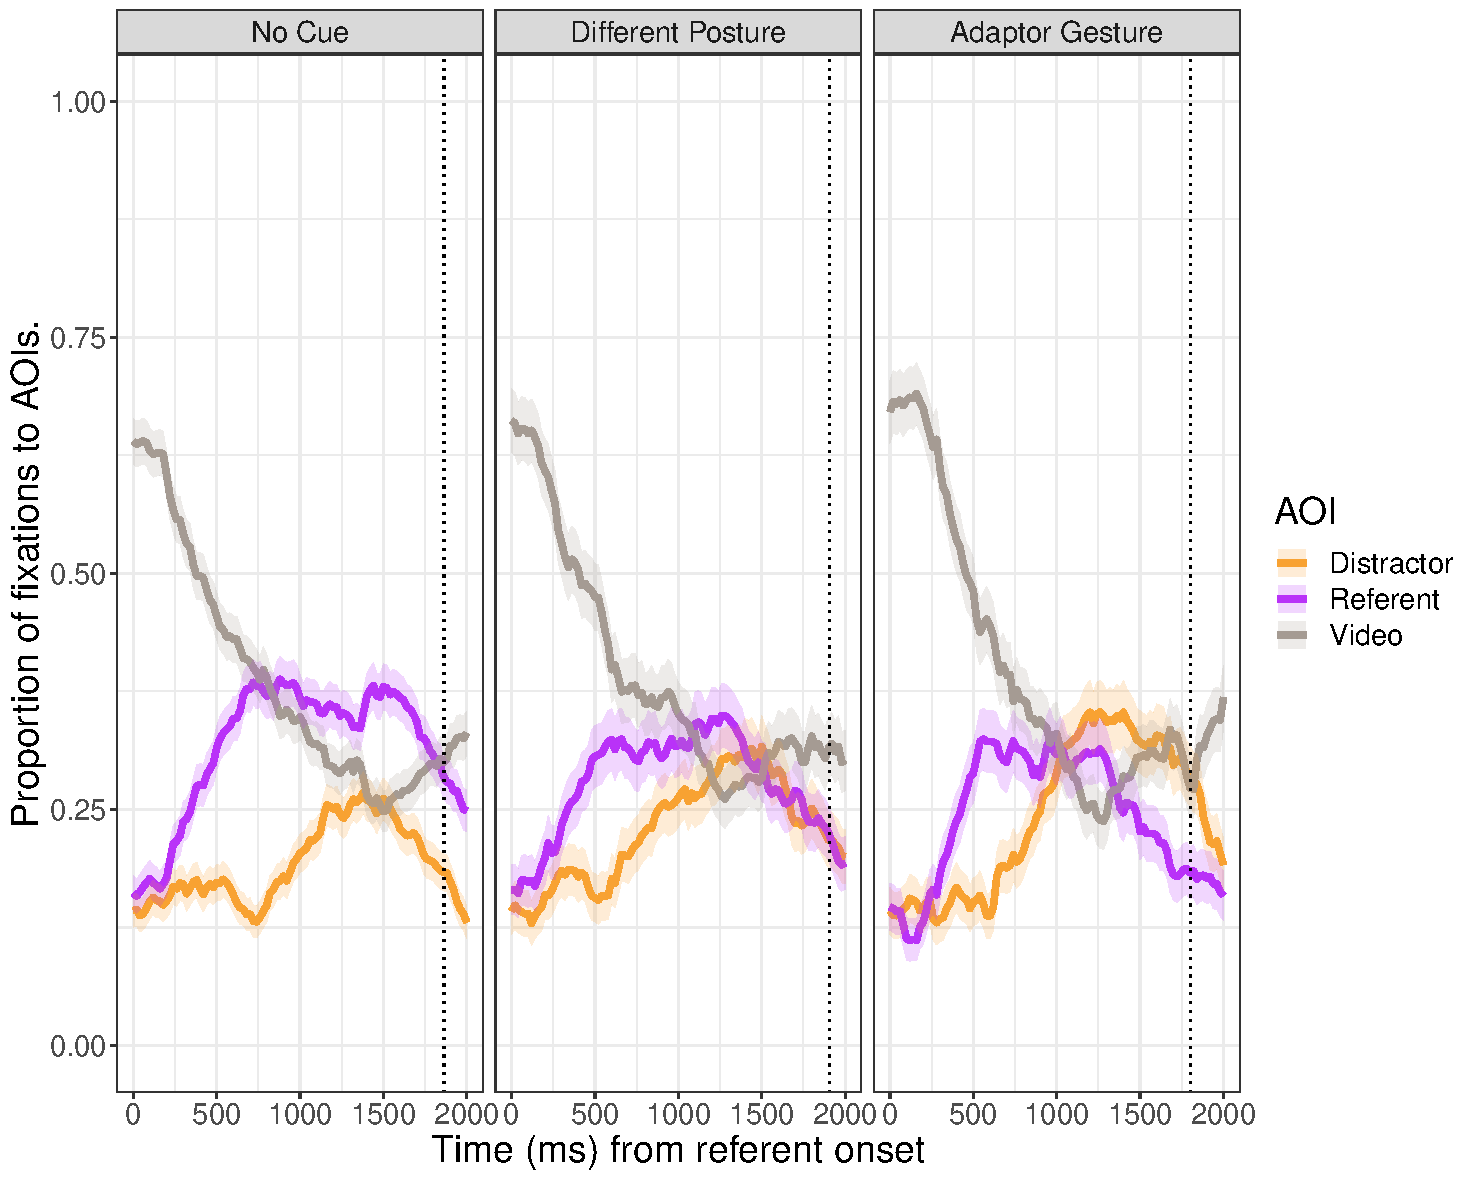
\includegraphics[width=\linewidth]{./img/e7_fixations_filler.pdf}
  \caption{Eye-tracking results for filler trials in Experiment~1: Proportion of fixations to each object (referent or distractor) and the video, from 0 to 2000 ms post-referent onset, calculated out of the total sum of fixations for each 20~ms time bin. Shaded areas represent $\pm$ 1 standard error of the mean.}
  \label{fig:v1_eye2}
\end{figure}


\subsection{Mouse movements}
Figure \ref{fig:v1_mouse2} shows the time course of the proportions of cumulative distance the mouse moved towards the referent and distractor in critical trials for 2000~ms from referent onset, split by each type of cue.
Analysis of mouse movements in filler trials also patterned with analysis of eye-movements for these trials:
Relative to videos showing no cue, the tendency to move towards the referent over the distractor (\resultsLM{1.08}{0.23}{4.62}) was significantly reduced for videos showing the speaker either in a different posture or producing an adaptor gesture (\resultsLM{-0.54}{0.12}{-4.52} and \resultsLM{-0.86}{0.12}{-7.19} respectively).

\begin{figure}[Ht]
  \centering
	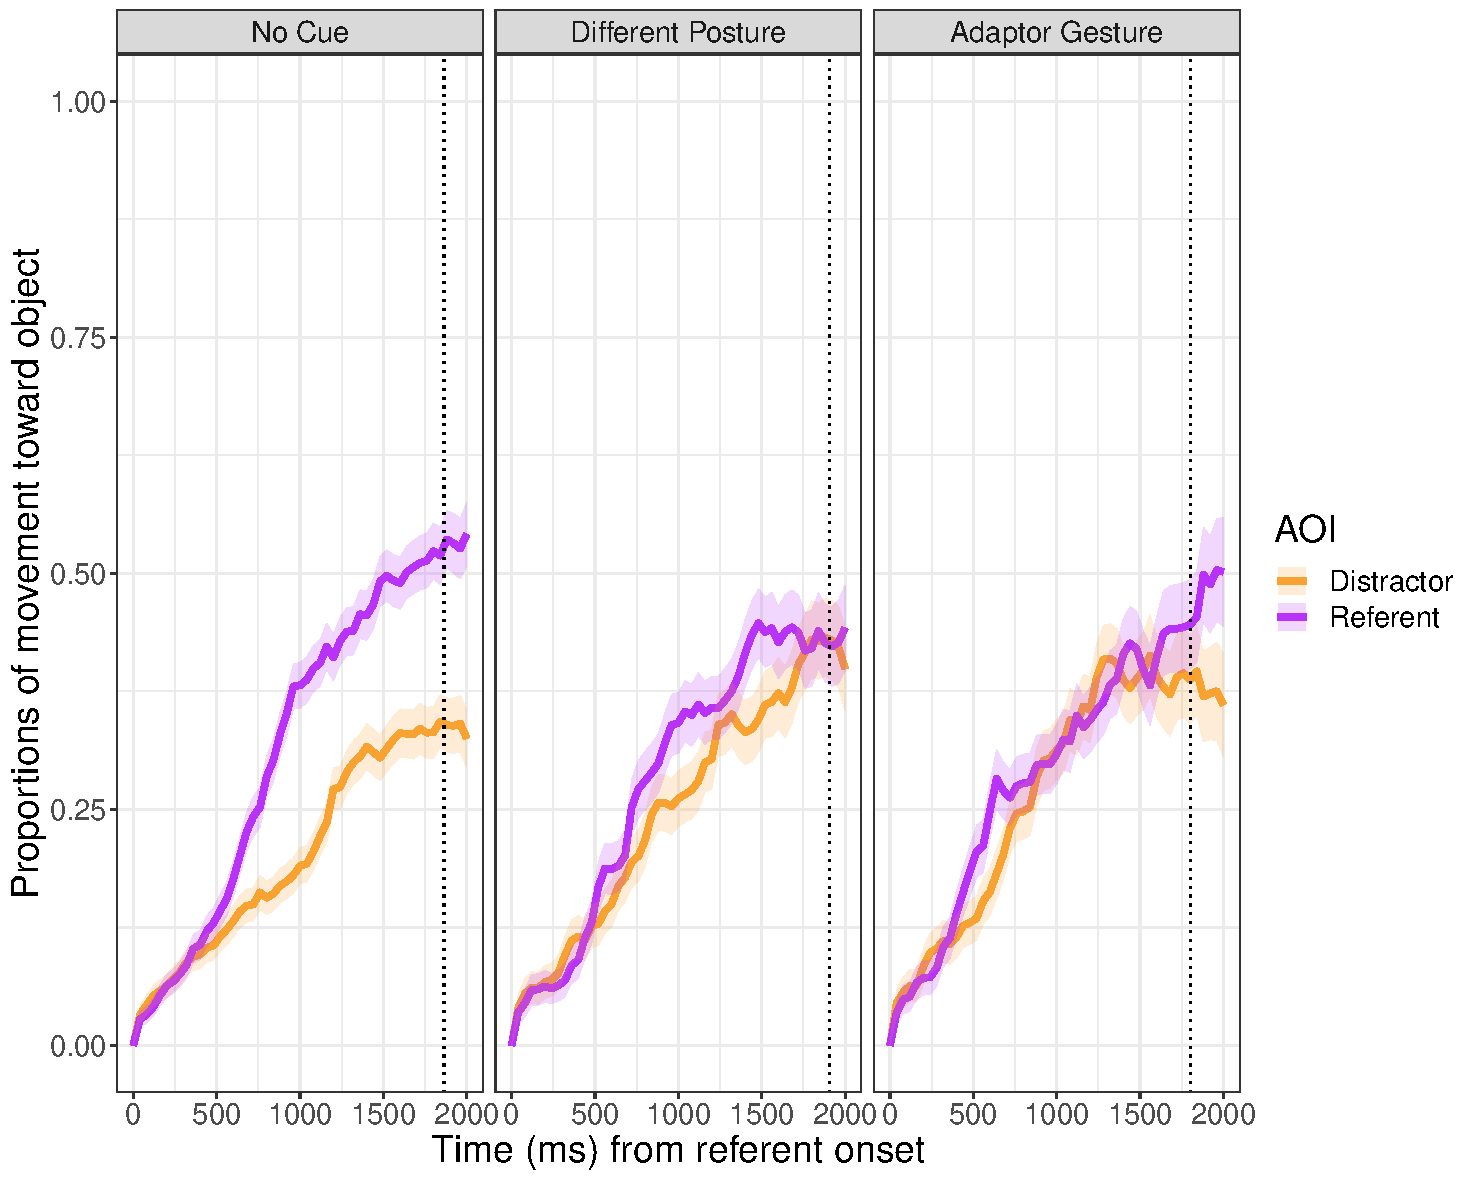
\includegraphics[width=\linewidth]{./img/e7_mouse_filler.pdf}
  \caption{Mouse-tracking results for filler trials in Experiment~1: Proportion of cumulative distance traveled toward each object from 0 to 2000 ms post-referent onset. Proportions were calculated from the total cumulative distance participants moved the mouse until that time bin (from video onset, when cursor was made visible). Shaded areas represent $\pm$ 1 standard error of the mean.}
  \label{fig:v1_mouse2}
\end{figure}


